\subsection{Diagramma delle classi del modello}

Le classi del modello sono le seguenti:
\begin{description}
\item[Game] classe statica che permette il caricamento dei dati di gioca da JSON e mantiene una referenza ai livelli e ai piatti

\item[Level] classe astratta, il metodo getNumberOfIngredientForDish ritorna il numero corretto di elementi solo per il Livello 1

\item[Dish] il piatto, un insieme di ingredienti

\item[Ingredient] l’ingrediente

\item[Turn] tiene traccia del completamento di un piatto, invia callback al relativo TurnListener. Al termine del piatto genera un TurnResult.

\item[TurnListener] interfaccia per la ricezioni di eventi relativi a un turno

\item[TurnResult] il risultato del turno
\end{description}

\begin{figure}[h!]
\centering{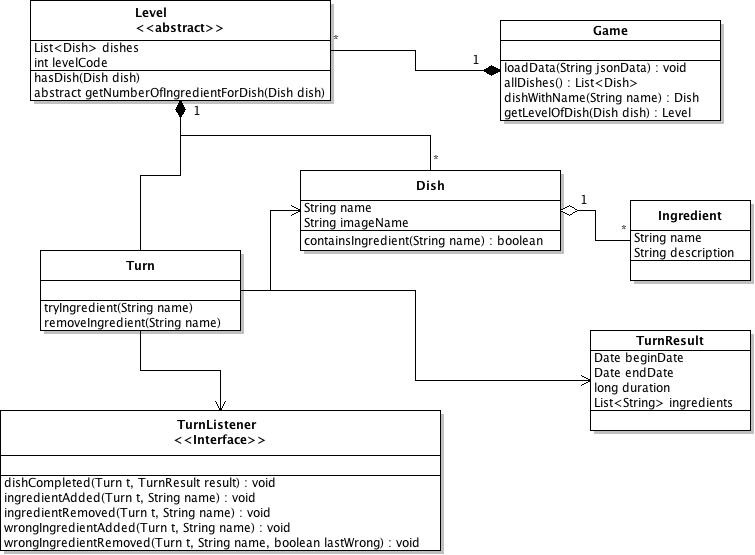
\includegraphics[width=\textwidth]{uml-class.jpg}}
\caption{Class Diagram}
\label{fig:uml}
\end{figure}

\subsection{AllJoyn}
La modalità multiplayer è stata realizzata attraverso AllJoyn. Qui si può trovare la documentazione completa: \url{https://allseenalliance.org/developers/develop/api-guide/core/android}.
L’applicazione espone un generico MultiPlayerService con il metodo \code{sendMessage()}. Questo metodo permette di inviare semplici Signal con un parametro stringa.
Il formato di invio dei messaggi è CSV, il primo elemento è il tipo del messaggio.
Verranno inviati tre tipi di messaggi:
\begin{enumerate}
\item dishes seguito dai nomi del piatti, rappresenta l’inizio del gioco, l’host della partita invia al joiner della sessione i piatti selezionati
\item stop inviato quando uno dei due dispositivi abbondona il gioco (alla ricezione di questo messaggio si torna indietro alla schermata principale)
\item dish seguito dal nome del piatto, indica il completamento di un piatto
\end{enumerate}

\subsection{Gimbal}
Nel gioco ciascun ingrediente è un trasmettitore Gimbal. Nell’applicazione si fa uso della versione 2 dell’API, in particolare si fa uso della parte di Beacon management. Qui la documentazione: \url{https://gimbal.com/doc/android/v2/devguide.html\#set\_beacon}
Tale API viene utilizzata nella MainActivity per orchestrare il flow del gioco. I beacon sono associati ad un ingrediente attraverso il name. La vicinanza di un beacon è determinata dal valore del suo RSSI. Il valore che discrimina la vicinanza di un beacon è -60. Attenzione: potrebbe essere necessario cambiare il threshold di vicinanza (si trova nella classe \code{Commons.java}).


\subsection{Activities}

L’applicazione dispone di quattro Activity:
\begin{description}
\item[StartActivity] mostra la schermata principale e carica i dati del gioco per evitare successivi caricamenti. Dispone di un bottone per l’inserimento della email per l’invio delle statistiche del gioco. La persistenza della email è affidata alle SharedPreferences di Android

\item[ChooseSessionActivity] mostra la schermata di scelta dei piatti, cerca nell’Intent un Extra “mode” che indica la modalità di gioco (singola o multiplayer). La selezione dei piatti può avvenire in due modi: selezionandoli da una GridView o premendo il tasto “Casuale”

\item[MultiPlayerConfigActivity] gestisce parte dall’inizializzazione della logica di AllJoyn, il comportamento varia a seconda se il giocatore seleziona di creare una partita (ruolo host) o di accedere ad una partita (ruolo joiner)

\item[MainActivity] orchestra la partita usando Gimbal API, AllJoyn Framework, la classe \code{Turn} e \code{TurnListener}. Cerca nell’Intent un Extra “mode” per la modalità e uno “dishes” per i piatti. 
\end{description}

Di seguito viene riportato il flow di accesso alle diverse activity.

\begin{figure}[h!]
\centering{
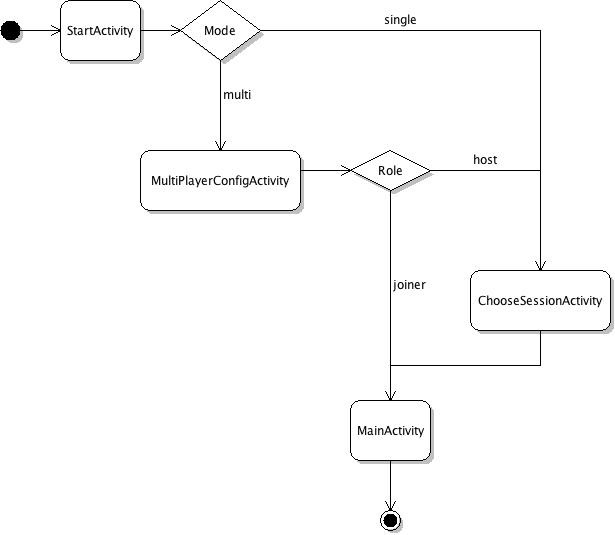
\includegraphics[width=\textwidth]{uml-activity1.jpg}}
\caption{Flow di accesso alle activity}
\label{fig:flow}
\end{figure}


Durante una partita il tasto Back di Android riporta alla schermata iniziale dopo una conferma. Nel caso di Multiplayer se un dispositivo abbandona la partita anche l’altro torna alla schermata principale.


\subsection{Adapters}

Per visualizzare liste di oggetti sono stati usati i seguenti Adapter:
\begin{description}
\item[DishAdapter] viene utilizzato nella schermata di selezione dei piatti, tiene traccia degli elementi selezionati

\item[IngredientAdapter] controlla la visualizzazione delle interazioni tra ingredienti e dispositivo. Mostra immagini diverse a seconda dell’assenza di ingredienti, ingredienti presenti o errati

\item[TableAdapter] controlla la visualizzazione della tavola con i sottopiatti vuoti o riempiti da quelli completati dalla squadra relativa al dispositivo e anche dalla squadra avversaria in caso di multiplayer.
\end{description}

Altre classi e file
\begin{description}
\item[Commons] contiene costanti, della logica condivisa durante il gioco (AllJoyn) e metodi statici (invio mail)

\item[GMailSender] e JSSEProvider classi helper per l’invio di email

\item[PrefUtils] classe helper per la gestione delle SharedPreferences

\item[\code{/raw/data.json}] file contente i dati del gioco (ingredienti, livelli, piatti)

\item[\code{/raw/data\_source.csv}] file originale in csv in cui erano contenuti i dati del gioco non ben strutturati

\item[\code{/raw/gen\_json.py}] script python per trasformare \code{data\_source.csv} in \code{data.json}
\end{description}
